\section{Tools voor het ontwikkelen van en een PWA}


\subsection{Lighthouse}

	Lighthouse is een tool die een audit zal uitvoeren op een website en een rapport zal uitgeven. Dit rapport kan een ontwikkelaar veel interessante informatie geven om de ervaring van deze website te verbeteren. De audit geeft inzichten op vlak van:
	
	\begin{itemize}
		\item	Prestaties
		\item	Toegankelijkheid
		\item	Best practices
		\item	SEO
		\item   PWA
	\end{itemize}
	
	\autocite{Lighthouse2020}
	
	Voor elk van deze onderdelen, op 'PWA' na, zal er een score op 100 gegenereerd worden. De audit zal ook voorstellen doen om deze scores te verhogen en de ervaring voor de eindgebruiker dus te verbeteren.
	
	Voor het onderdeel PWA zal er een checklist gegenereerd worden met items die moeten voldaan worden zodat de applicatie geïnstalleerd kan worden op een toestel. Dit onderdeel wordt opgedeeld in drie delen: “fast and reliable”, “installable” en “PWA optimized”.
	
	
	\subsubsection{Fast and reliable}
		De eerste metriek die getest wordt, is de snelheid van de website. Er wordt zowel gekeken naar de snelheid waarmee de eerste inhoud op de pagina komt (FMP – first meaningful paint) maar ook naar wanneer de gebruiker voor het eerst kan interageren met de website (TTI – time to interactive).
		\autocite{web.dev2020}
		
		Vervolgens worden de offline capaciteiten van de website getest. Er wordt getest als de huidige pagina en startpagina reageren met een antwoord die de statuscode 200 bevat. Dit wil zeggen dat er een succesvol antwoord was en dat de website dus offline kan werken.
	
	
	\subsubsection{Installable}
	
		In dit deel van de PWA-audit zal gecontroleerd worden of als de website voldoet aan alle vereisten om geïnstalleerd te kunnen worden. Dit zijn:
		\begin{itemize}
			\item	Er moet een HTTPS-verbinding zijn.
			\item	Er moet een service worker geregistreerd worden.
			\item	Er moet een minimum app-manifest zijn.
		\end{itemize}
		\autocite{web.dev2020a}
		
	
	\subsubsection{PWA optimized}
	
		In dit onderdeel wordt er gecontroleerd op kleine optimalisaties die een betere gebruikers-ervaring kunnen bieden. 
		Een voorbeeld hiervan is dat als een gebruiker naar de HTTP-versie van een website surft, hij herleid wordt naar de https-versie.
		
		Een andere controle is dat het themakleur van de applicatie is ingesteld. Dit kan gebeuren in de app-manifest. Ook dit zorgt voor een betere user experience en een meer native feeling. Deze app manifest moet een specifiek icoon bevatten voor de IPhone. Ook deze controle wordt uitgevoerd.
		
		
		\begin{figure}[H]
			\centering
			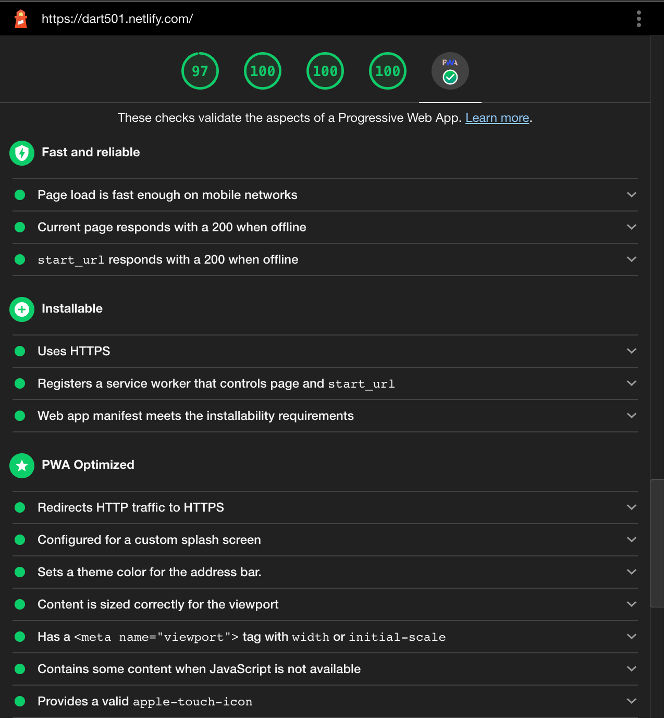
\includegraphics{./img/lighthouse.png}
			\caption{screenshot van het onderdeel 'PWA' in een lighthouse audit op de site \href{ https://dart501.netlify.com}{dart501.netlify.com} }
		\end{figure}
		
		

\subsection{Workbox}

	Workbox is een verzameling van libraries die helpt bij het ontwikkelen van service worker gerelateerde functionaliteiten.
	
	Workbox wil het gemakkelijker maken voor de ontwikkelaars om middelen te cachen en op deze manier een snellere en minder netwerk-afhankelijke applicatie te maken.
	
	Het debuggen van een PWA kan ook moeilijk worden omdat code lokaal opgeslagen kan worden en je als ontwikkelaar niet altijd weet welke versie van de code voor een bepaald gedrag zorgt. Ook om deze problemen te debuggen voorziet Workbox tools.
	\autocite{Workbox2020}
	

\subsection{PWAbuilder}

	Pwabuilder.com is een website, die gecreëerd werd door Microsoft, die ervoor zorgt dat een PWA toch in de app-stores kan terechtkomen. Als ontwikkelaar moet je juist een link van een PWA opgeven en de tool maakt van deze PWA vier pakketten die kunnen geüpload worden naar hun bijhorende app-store. 
	
	Volgende platformen zijn ondersteund:
	-	Android
	-	Samsung (eigen Samsung store)
	-	Windows
	-	IOS
	
	\begin{itemize}
		\item	Android
		\item	Samsung (eigen Samsung store)
		\item	Windows
		\item	IOS
	\end{itemize}
	\autocite{PWAbuilder2020}
	
	
\subsection{Chrome developer tools}
	De Chrome developer tools bieden een grote hulp bij het ontwikkelen van webapplicaties.
	
	Chrome zorgt ervoor dat er eenvoudig gecachete items tijdelijk verwijderd kunnen worden. Hierdoor kan de ontwikkelaar testen als een service worker de juiste bestanden offline beschikbaar maakt.
	
	Google Chrome biedt tools om eenvoudig een website offline te testen of om bepaalde service workers uit te schakelen.
	Ook de volledigheid van het app-manifest bestand kan in de Chrome developer tools bekeken worden
	
	De chrome devloper tools hebben ook een sectie waar de status van de service worker kan bekeken en gemanipuleerd worden.
	\autocite{Developers2019b}
	

	
	